\section{问题及解决方案}

\subsection{不同源影像色彩不同}
超分影像要求低分辨率影像和高分辨率影像色调一致, 不能一明一暗. 因此需要通过直方图匹配的方式将S2影像色调调整至与GF-1相似. 使用\href{http://blog.sina.com.cn/s/blog_764b1e9d0102vqws.html}{ENVI扩展工具:直方图匹配工具}, 遇到报错如图~\ref{fig:0201}所示: 

\begin{figure}[!htbp]
    \centering
    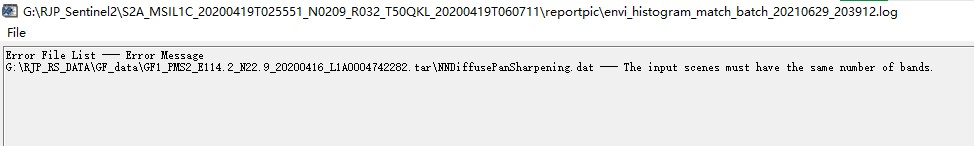
\includegraphics[height=5em]{pic/q0100a.jpg}
    \caption{报错一: 波段数量}
    \label{fig:0201}
\end{figure}

其报错为波段数目不同, 因此将GF-1四个波段通过波段拆分, 再将RGB三个波段进行合成, 得到与S2相同波段数的图像. 又遇到问题, 如图~\ref{fig:0202}所示. 

\begin{figure}[!htbp]
    \centering
    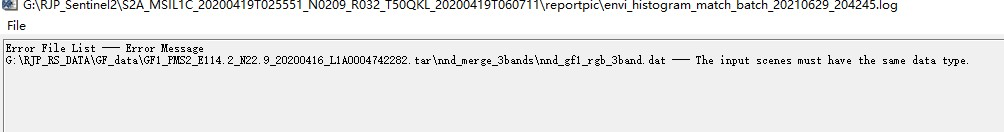
\includegraphics[height=4em]{pic/q0100b.jpg}
    \caption{报错二: 数据类型}
    \label{fig:0202}
\end{figure}

猜想是否因为无效数据的原因, 目前已尝试裁剪相同小块图像进行直方图匹配, 仍然报错. 说明确实是数据类型问题因此导致插件无法使用. 经了解遥感数据类型主要为每个像素的数据类型, float(浮点型), int(整型), uint(无符号整型)等, 代表着每个像素值的取值范围. GF1影像数据类型为int, 数据范围为-2147483648($-2^{31}$)到2147483648($2^{31}$), S2影像数据类型为uint, 数值范围为0到4294967295($2^{32}$). 在这里猜想, 直方图匹配使用的是RGB值, 而遥感影像一般使用反射率进行拉伸得到RGB值, 显然不同的遥感数据类型需要进行转换才可以进行直方图匹配, ENVI直方图匹配插件本应考虑这一点, 但却没有, 因此需要进行数据格式的转换, 如图~\ref{fig:0203}所示.

\begin{figure}[!htbp]
    \centering
    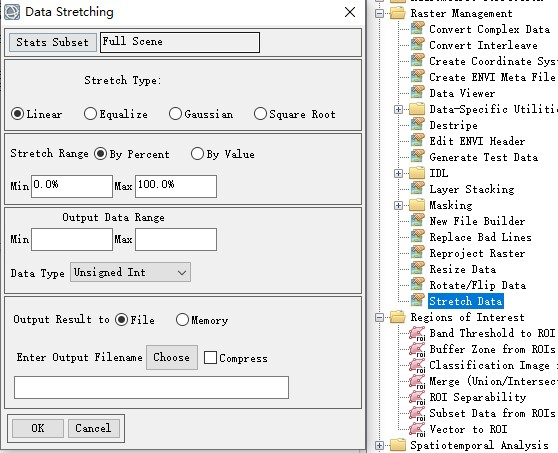
\includegraphics[width=0.7\textwidth]{pic/q0101.jpg}
    \caption{ENVI数据类型转换}
    \label{fig:0203}
\end{figure}

转换后的结果如图~\ref{fig:0204}所示, 影像中存在黑色无效数据, 且因为无效值影响, 影像整体变色严重. 首先通过编辑头文件信息(见20210630报告)将无效值设为0, 之后, 影像并未发生变化; 使用ENVi的Cursor Value工具对黑色无效数据进行取值, 其值为 ``1857, No Data, 9138''. 此时修改头文件并无作用, 猜想, 是否当所有波段值皆为 ``No Data, No Data, No Data''时, 修改头文件将无效值设置为0, 才能有效剔除黑色无效数据. 

\begin{figure}[!htbp]
    \centering
    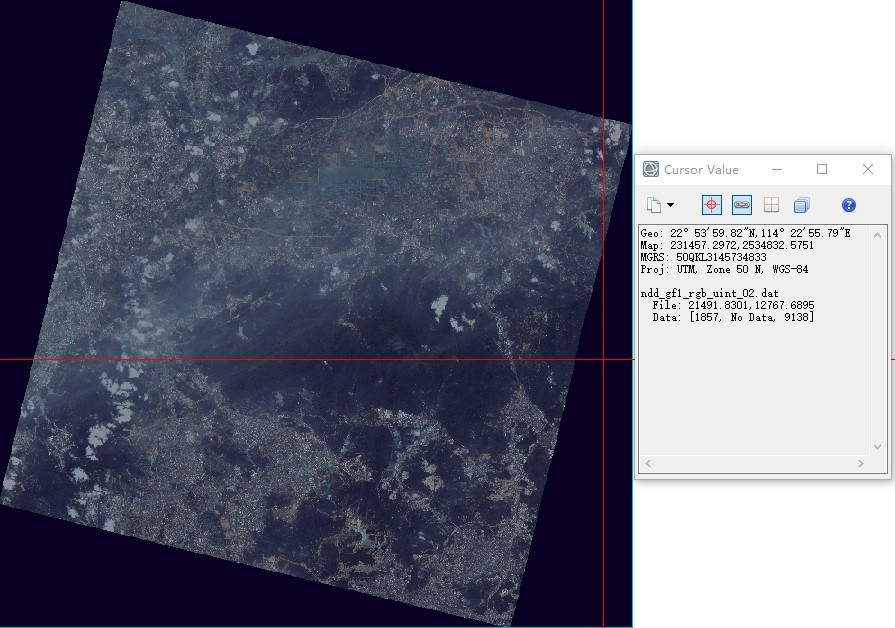
\includegraphics[width=0.7\textwidth]{pic/q0102.jpg}
    \caption{转换后影像无效数据}
    \label{fig:0204}
\end{figure}

分析过程. 现在存在两个问题, 一是黑色无效数据, 二是影像变色. 仔细思考, 发现正是黑色无效数据引起影像变色. 对于黑色无效数据, 之前处理的波段值皆为 `No Data, No Data, No Data'', 操作时将其设置为 ``0, 0, 0''. 那么能否直接将黑色数据设为 ``0, 0, 0'', 这样是否可以同时解决无效数据与影像变色问题. 那么如何将 ``1857, No Data, 9138'' 变为 ``0, 0, 0'', 使用ENVI波段运算工具, 分别进行 ``band1-9138'', ``band2+0'', ``band3-1857'', 其生成的三个波段如图~\ref{fig:0205}所示.

\begin{figure}[!htbp]
    \centering
    \subfloat[]{\label{fig:0205a}
    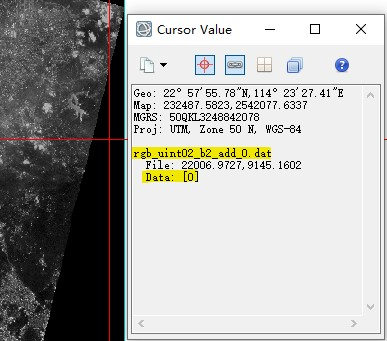
\includegraphics[width=10em]{pic/q0103.jpg}}
    \quad
    \subfloat[]{\label{fig:0205b}
    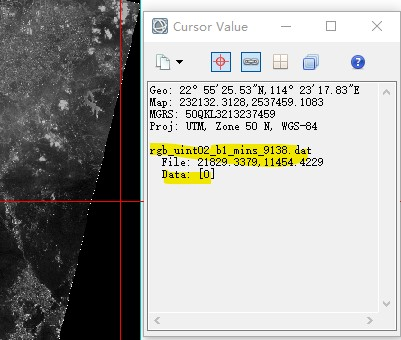
\includegraphics[width=10em]{pic/q0104.jpg}}
    \quad
    \subfloat[]{\label{fig:0205c}
    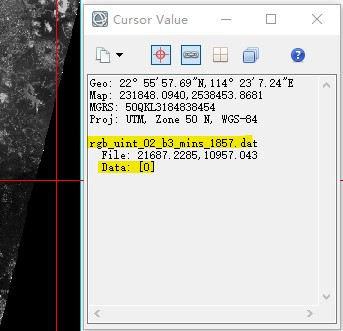
\includegraphics[width=10em]{pic/q0105.jpg}}
    \caption{波段运算结果}
    \label{fig:0205}
\end{figure}

之后进行波段合成, 虽也得到黑色无效数据, 但通过编辑头文件将其无效值设置为0可完成无效数据剔除, 同时影像色调和原始影像一样, 如图~\ref{fig:0206}所示. 

\begin{figure}[!htbp]
    \centering
    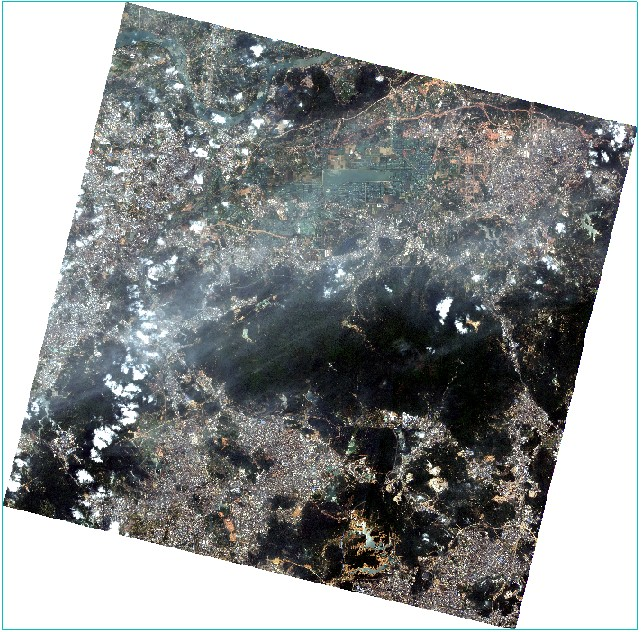
\includegraphics[height=16em]{pic/q0106.jpg}
    \caption{影像数据格式转换最终结果}
    \label{fig:0206}
\end{figure}

之后进行S2影像与GF影像的直方图匹配, 整幅图像匹配前后结果如~\ref{fig:0207}所示:

\begin{figure}[!htbp]
    \centering
    \subfloat[匹配前]{\label{fig:0207a}
    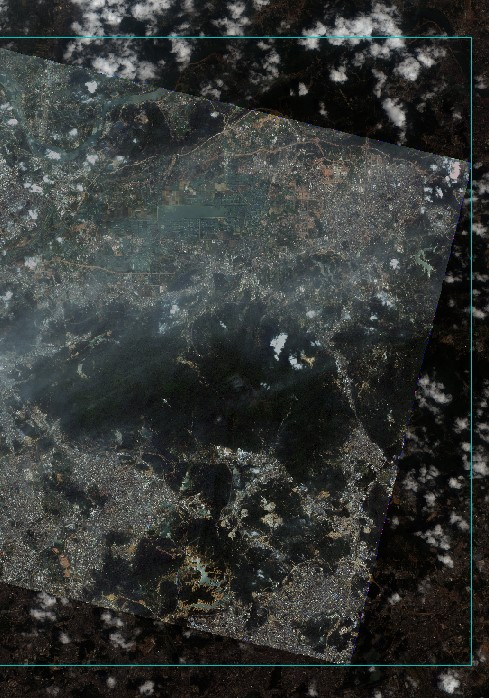
\includegraphics[height=20em]{pic/q0108.jpg}}
    \qquad
    \subfloat[匹配后]{\label{fig:0207b}
    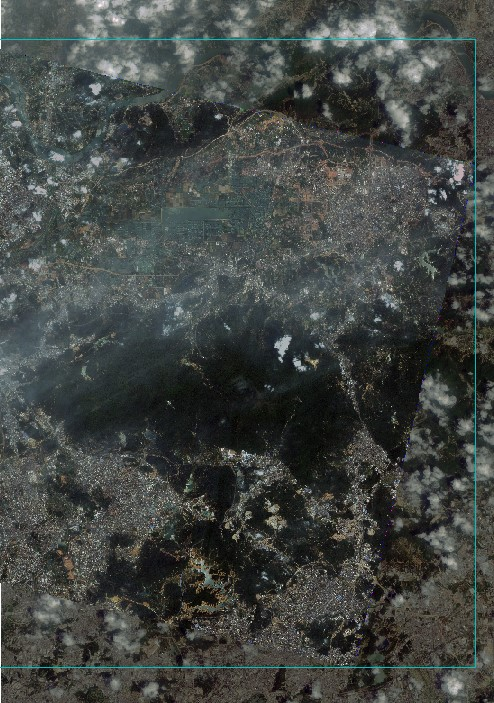
\includegraphics[height=20em]{pic/q0107.jpg}}
    \caption{直方图匹配结果对比}
    \label{fig:0207}
\end{figure}

其整体效果匹配非常好, 但高分影像数据及不会使用整幅影像最为一对, 需要进行裁剪, 直方图匹配后的局部效果如图~\ref{fig:0208}所示, 其差异极大. 

\begin{figure}[!htbp]
    \centering
    \subfloat[匹配前]{\label{fig:0208a}
    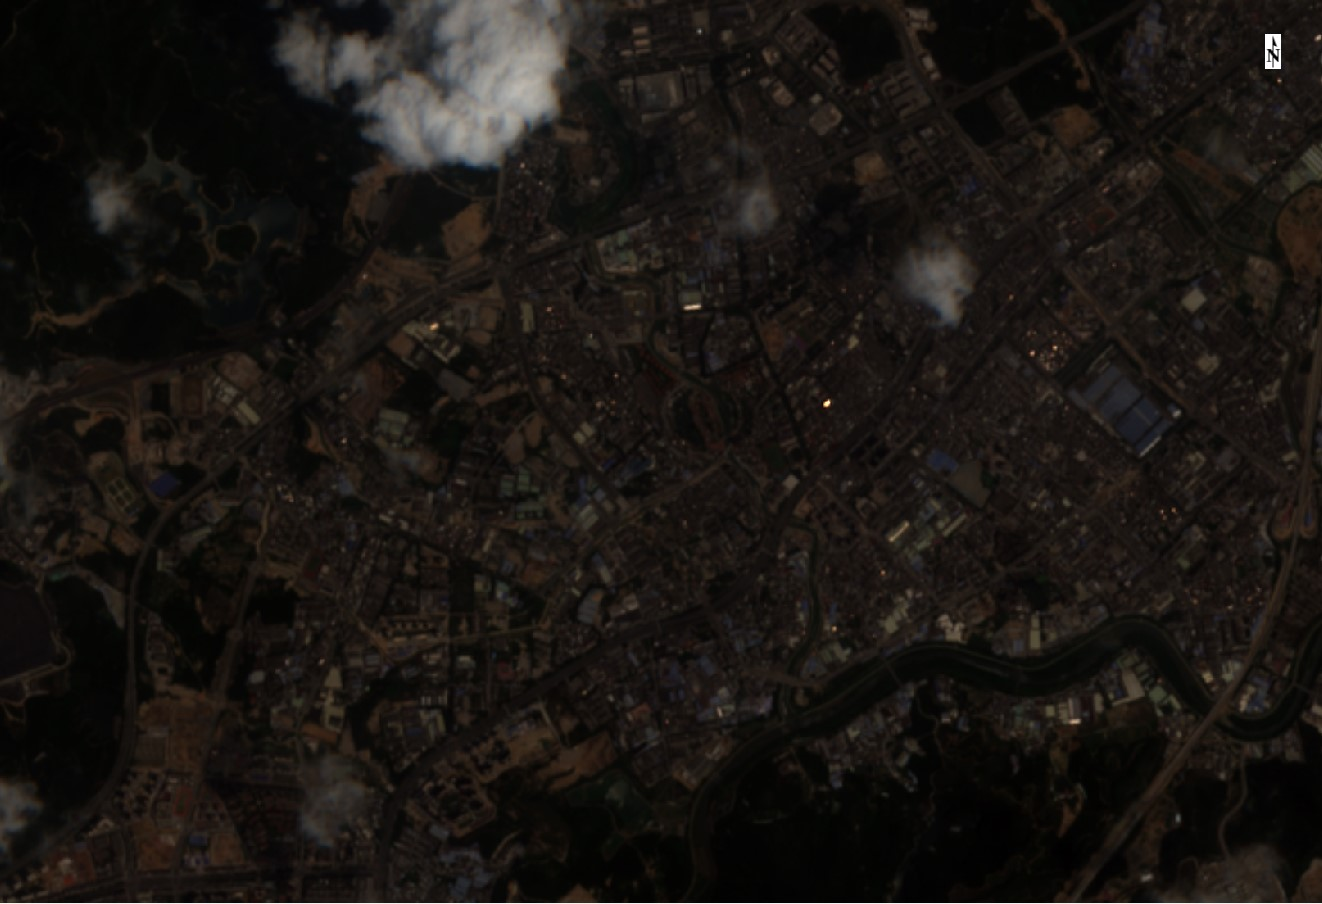
\includegraphics[height=10em]{pic/q0109.jpg}}
    \qquad
    \subfloat[匹配后]{\label{fig:0208b}
    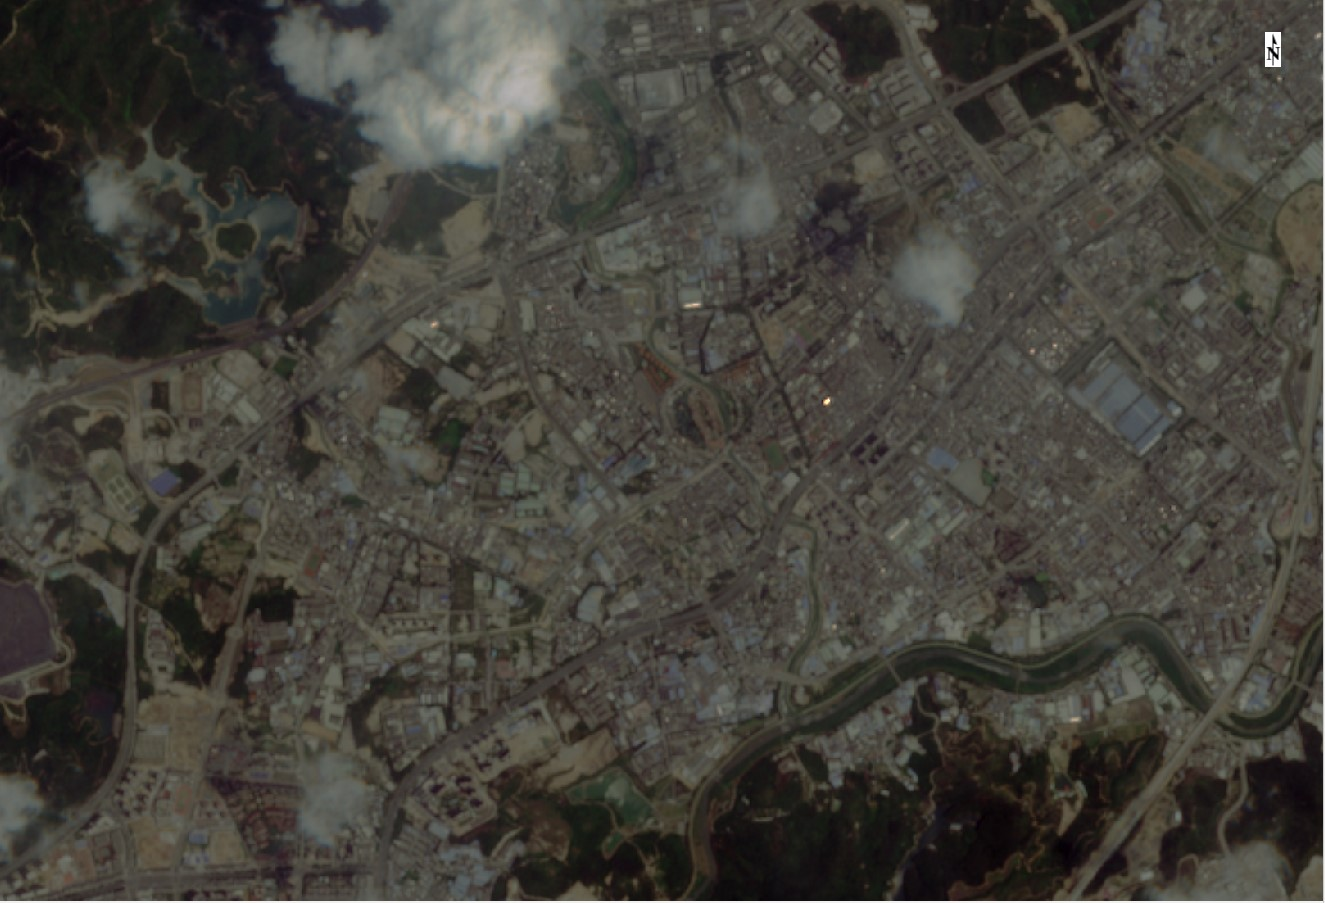
\includegraphics[height=10em]{pic/q0110.jpg}}
    \caption{局部直方图匹配结果对比}
    \label{fig:0208}
\end{figure}

对此的思考有: 
\begin{itemize}
    \item 整幅影像进行直方图匹配后, 不能直接裁剪用于超分影像集.
    \item 为了数据集制作效率, 也不可能使用ENVi将整幅影像裁成小块影像, 一个个进行直方图匹配. 
    \item 为保证效率, 应先进行批量小块裁剪, 为了保证数据集每对图像的色调一致, 最后对裁剪后的每一对高低分辨率影像进行直方图匹配.
\end{itemize}

\subsection{大块影像裁剪中精匹配遗留问题}
因此, 为了提高数据集制作效率, 先将进行大块的影像裁剪, 保存成png图像, 之后对png图像进行批量裁剪. 这是影像集制作的思路. 

再进行大块裁剪时, 选择ROI(region of interest)发现低分辨率的S2影像和高分辨率GF影像, 截取出的影像分辨率相同, 显然不正常. 通过一步步追查, 发现在影像匹配中, 对匹配影像的分辨率进行了2m $\times$ 2m 的重采样. 需要在图~\ref{fig:0209}所示, 对其分辨率进行设置, 将 ``Output Pixel Size From'' 设置为 ``Warp Image'', 之前错误的设置为 ``Base Image''.

\begin{figure}[!htbp]
    \centering
    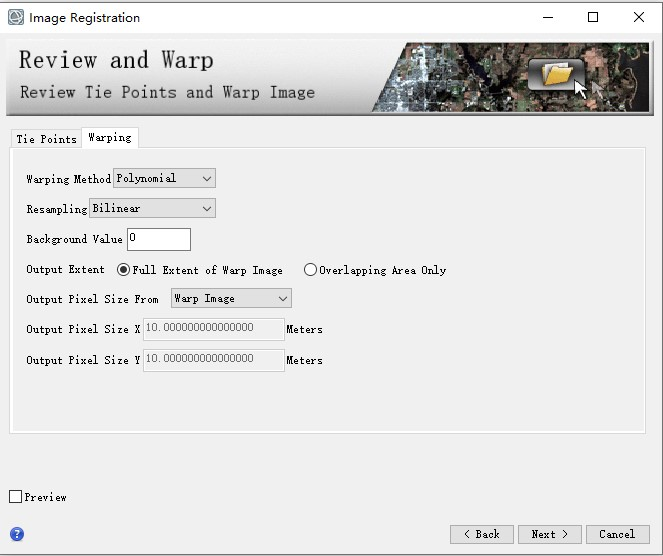
\includegraphics[height=15em]{pic/q0202.jpg}
    \caption{影像匹配分辨率正确设置}
    \label{fig:0209}
\end{figure}

与此同时又进行了一次影像匹配, 观察其同名点分布, 如图\ref{fig:0210}.

\begin{figure}[!htbp]
    \centering
    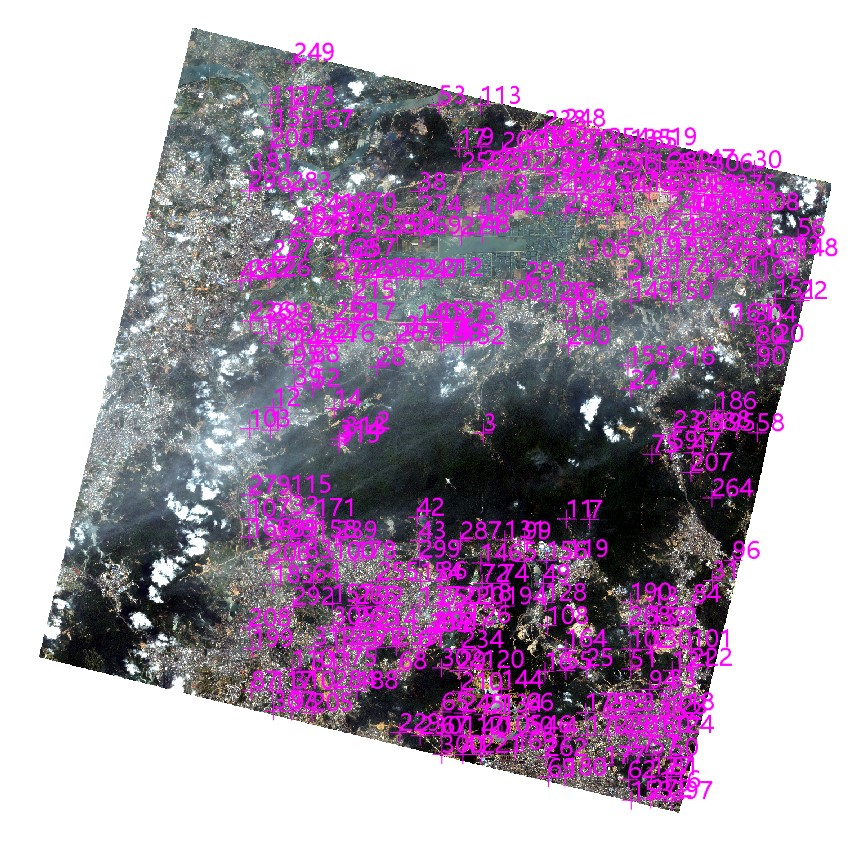
\includegraphics[height=20em]{pic/q0201.jpg}
    \caption{影像精匹配同名点分布}
    \label{fig:0210}
\end{figure}

发现在山区(同名点少的地方)出现偏差, 即影像不重叠. 手动在山区勾选了十个左右的同名点再进行影像精匹配 低分辨率S2影像和高分辨率GF影像依然存在一定偏差, 大致有20米左右, 如图~\ref{fig:0211}所示

\begin{figure}[!htbp]
    \centering
    \subfloat[GF局部山区影像]{\label{fig:0211a}
    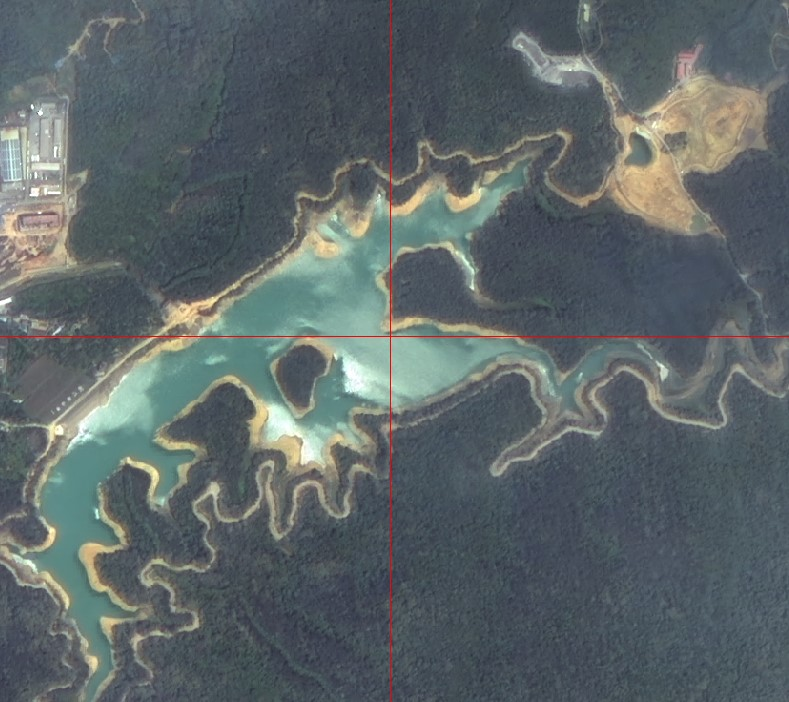
\includegraphics[height=10em]{pic/q0203.jpg}}
    \qquad
    \subfloat[S2局部山区影像]{\label{fig:0211b}
    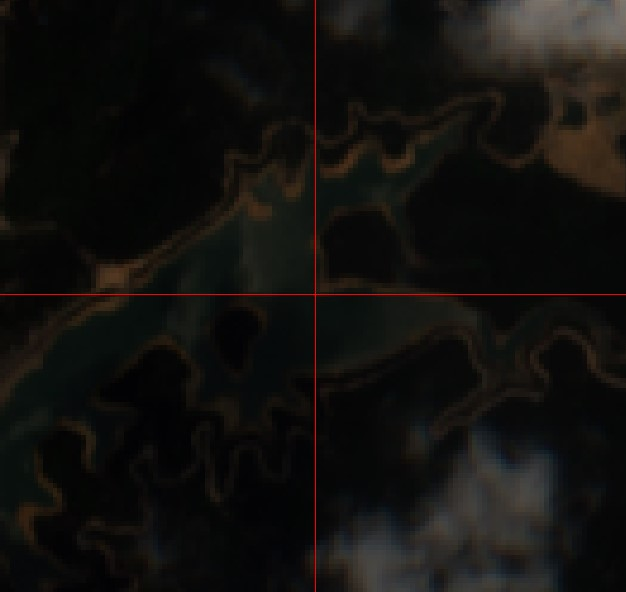
\includegraphics[height=10em]{pic/q0204.jpg}}
    \caption{局部直方图匹配结果对比}
    \label{fig:0211}
\end{figure}

影像匹配, 同名点稀疏之处匹配精度不高, 这也符合影像匹配的规律, 因此大块裁剪多在同名点多的区域, 如城市区域, 裁剪区域如图~\ref{fig:0200}

\begin{figure}[!htbp]
    \centering
    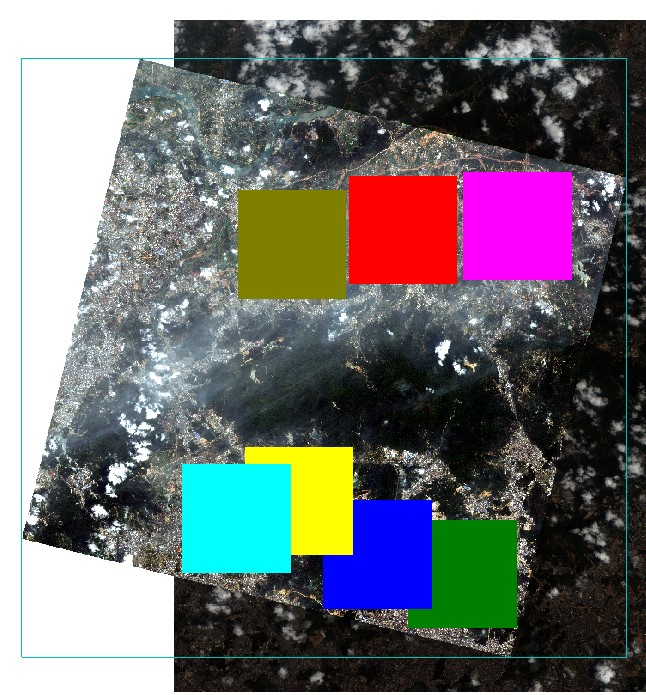
\includegraphics[height=20em]{pic/q0200.jpg}
    \caption{影像精匹配同名点分布}
    \label{fig:0200}
\end{figure}

分别以4000 $\times$ 4000和 800 $\times$ 800 的大小对GF影像和S2影像同名点密集区域进行裁剪. 发现裁剪出影像分辨率总是4001 $\times$ 4001和 801 $\times$ 801, 如图~\ref{fig:0212}. 参考\href{http://blog.sina.com.cn/s/blog_764b1e9d01016zgd.html}{ENVi下让两幅图像行列大小一致的方法}得出其产生的原因大致为, 精度取舍, 比如矢量边界刚好落在一个图像上半个像元的位置, 而另外一个图像上是落在$\frac{3}{4}$个像元处, 这种情况下裁剪结果的行列大小不一致. 解决方法是直接通过图像二次裁剪去掉即可.

\begin{figure}[!htbp]
    \centering
    \subfloat[ROI分辨率]{\label{fig:0212a}
    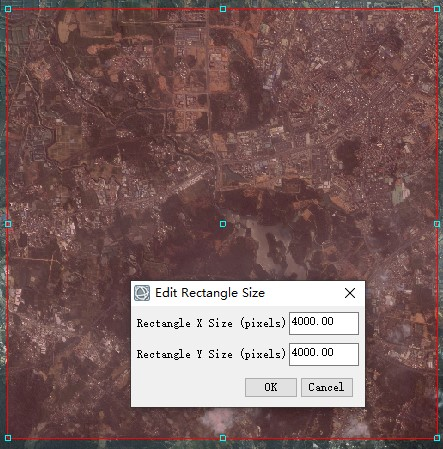
\includegraphics[height=10em]{pic/q0303.jpg}}
    \qquad
    \subfloat[裁剪后分辨率]{\label{fig:0212b}
    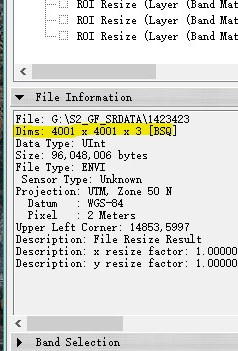
\includegraphics[height=10em]{pic/q0304.jpg}}
    \caption{局部直方图匹配结果对比}
    \label{fig:0212}
\end{figure}

\subsection{影像拉伸}

在整体裁剪后, 发现不同影像拉伸方式对影像的细节影响很大, 以高分影像为例, 使用optimized linear拉伸和linear 2\%拉伸的结果如图~\ref{fig:0213}所示.

\begin{figure}[!htbp]
    \centering
    \subfloat[optimized]{\label{fig:0213a}
    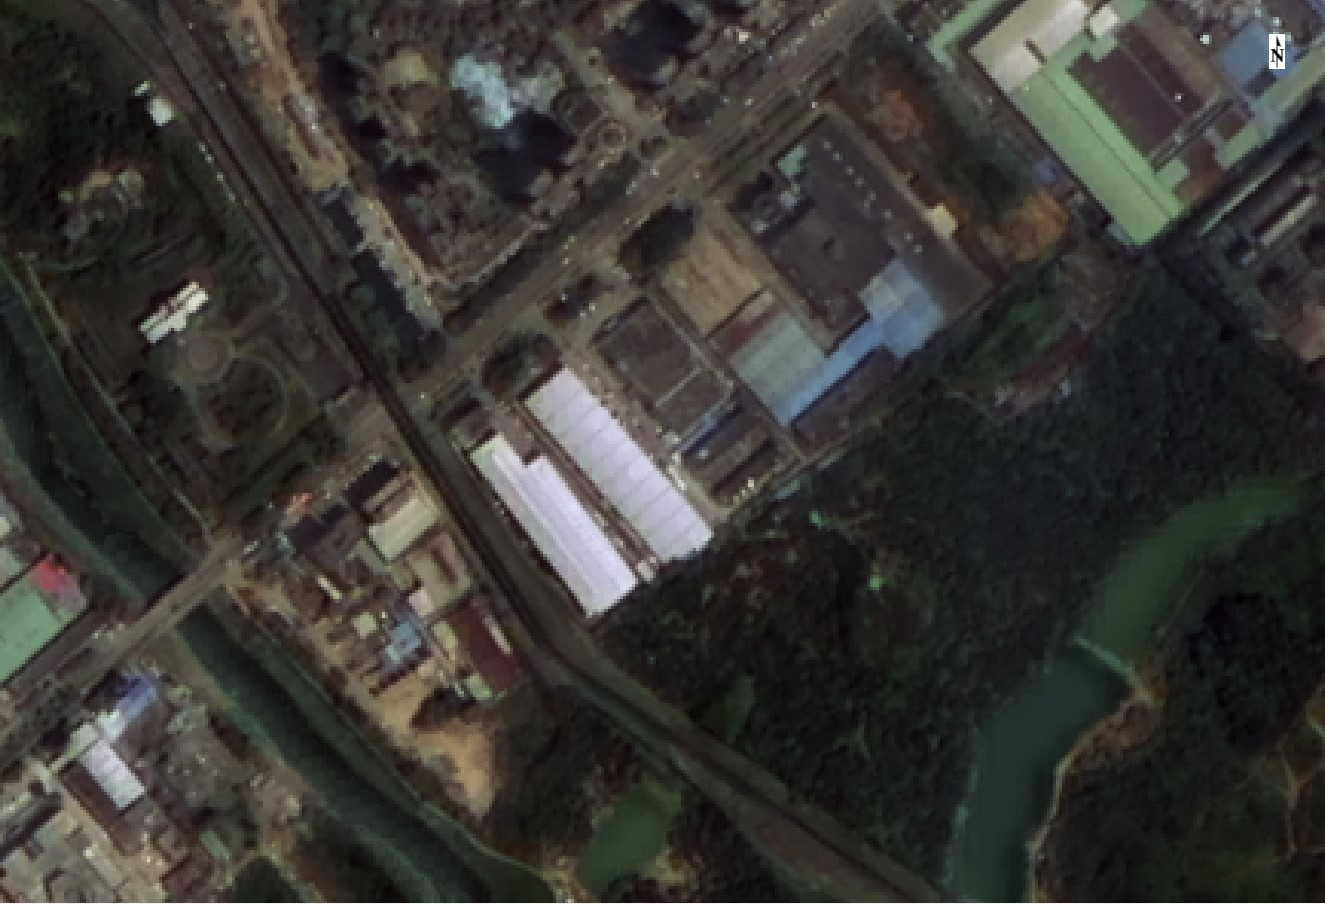
\includegraphics[height=10em]{pic/q0301.jpg}}
    \qquad
    \subfloat[linear 2\%]{\label{fig:0213b}
    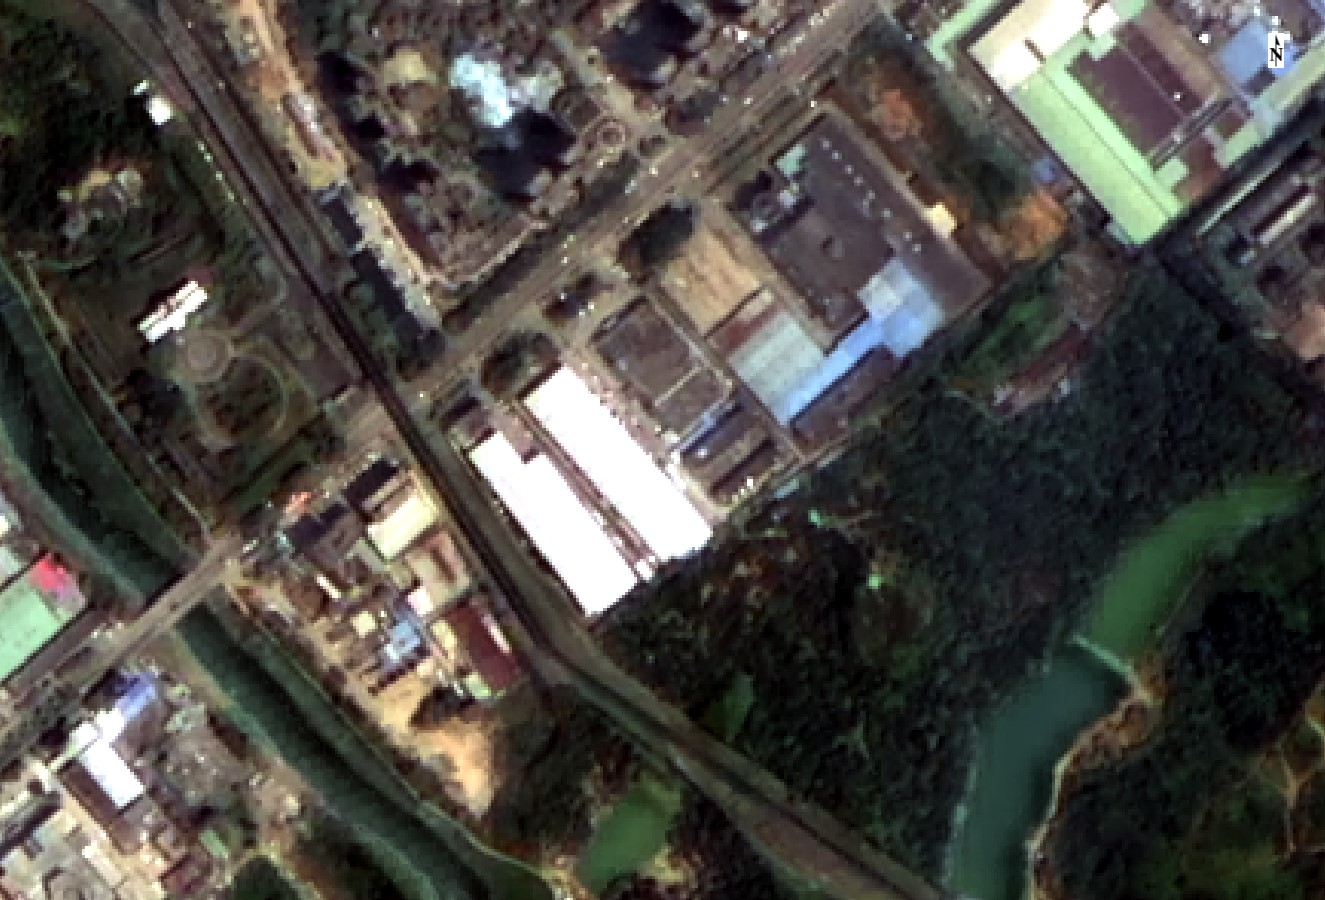
\includegraphics[height=10em]{pic/q0302.jpg}}
    \caption{两种拉伸效果对比}
    \label{fig:0213}
\end{figure}

可发现, linear2\%拉伸时, 图像整体变亮, 同时白色房子的纹理部分丢失, 但同时道路边界更加明显. 每一种拉伸都是一种对图像某种特征的取舍. 经过多种人眼直观感受, 个人认为 optimized linear的效果时最均衡的. 

同时对ENVI几种常见的拉伸方式进行介绍.

\begin{itemize}
    \item Linear Stretch (2\%)
    \item Optimized Linear Stretch
    \item Equalization Stretch 
    \item Guassian Stretch
\end{itemize}

遥感光学影像三个波段并非直接RGB值, 而是经过预处理的地物反射率. ENVi在显示遥感影像时, 将最低反射率作为0的灰度值, 将最高反射率最为255, 进行线性拉伸, 这是最普通的Linear Stretch影像显示方式. 如果不对遥感影像进行拉伸, 则显示效果为全黑或者全白. 那么Linear 2\%的拉伸, 则是将直方图中过低过高的值剔除. 先对遥感影像进行直方图统计, 将0-2\%的像素值设为0, 将98\%-100\%的像素值设为255. Linear 1\%和Linear 5\%也相同. 

而Optimized Linear Stretch则更复杂, 它与Linear Stretch相似, 但设置了更多参数确保影像中间值, 阴影, 高光部分到达一种均衡. 在ENVI中, Optimized Linear Stretch中有默认的四个参数, 无法更改:
\begin{itemize}
    \item Min Percent 0.025
    \item Max Percent 0.99
    \item Min Adjust Percent 0.1
    \item Max Adjust Percent 0.5
\end{itemize}


首先统计影像的累计直方图, $a$为min percent对应的像素值, $b$为max percent的像素值. 通过着$c$和$d$, OLS设置了新的min和max值进行线性拉伸, 其计算公式如~\ref{eq0201}和~\ref{eq0202}所示. 

\begin{equation}
    c = a - 0.1(b - a)
    \label{eq0201}
\end{equation}

\begin{equation}
    d = b + 0.5(b - a)
    \label{eq0202}
\end{equation}

其中0.1为 ``Min Adjust Percent'', 0.5为 ``Max Adjust Percent'', 以新计算出的 $c$和$d$为最小值和最大值进行线性拉伸, 便可得到Optimized Linear Stretch结果. 其直方图结果如~\ref{fig:0214}

\begin{figure}[!htbp]
    \centering
    \subfloat[optimized]{\label{fig:0214a}
    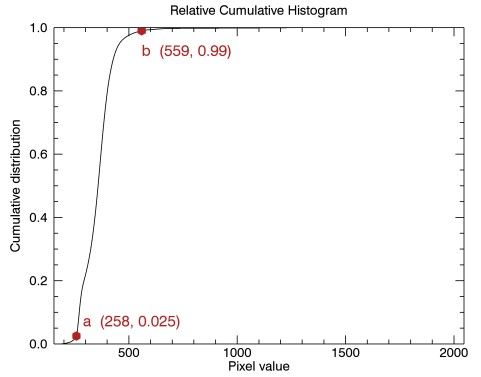
\includegraphics[height=10em]{pic/q0305.jpg}}
    \qquad
    \subfloat[linear 2\%]{\label{fig:0214b}
    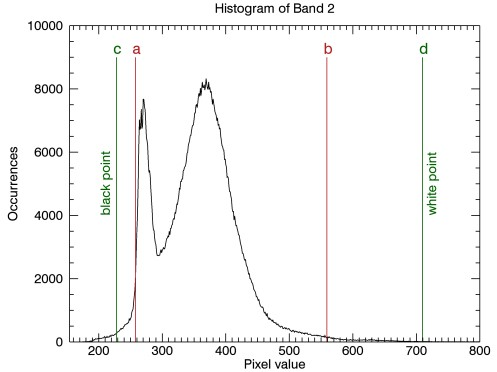
\includegraphics[height=10em]{pic/q0306.jpg}}
    \caption{两种拉伸效果对比}
    \label{fig:0214}
\end{figure}

而Guassian Stretch是将显示颜色的均值设置为127, 大于三倍中误差的像元分别将其像素值设置为0和255, 其他中间值用高斯曲线进行变换得到. Equalization Stretch则是对影像做直方图均衡化. 

\subsection{地理坐标系统分析}
对遥感影像预处理后, 需要进行精匹配. 其原因是同一地物在几何校正后的不同源影像中经纬度有微小差异, 该子章节对其投影方式进行了分析. 在ENVI查看GF和S2影像的坐标系, 如图~\ref{fig:0215}所示.

\begin{figure}[!htbp]
    \centering
    \subfloat[GF影像]{\label{fig:0215a}
    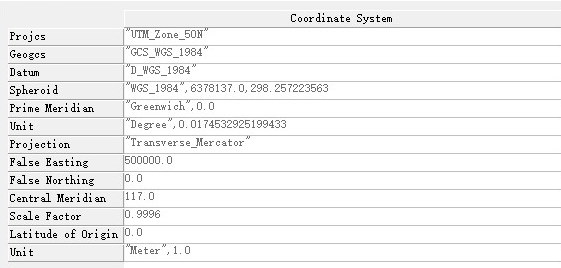
\includegraphics[height=10em]{pic/q0401.jpg}}
    \\[12pt]
    \subfloat[S2影像]{\label{fig:0215b}
    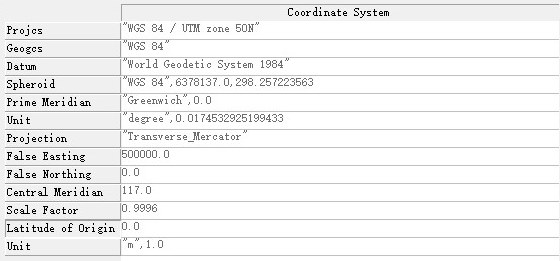
\includegraphics[height=10em]{pic/q0403.jpg}}
    \caption{坐标系信息}
    \label{fig:0215}
\end{figure}

发现其投影坐标系(Projcs), 地理坐标系(Geogcs), 和大地基准面(Datum)名称上的不同(参考\href{https://blog.csdn.net/ivan_ljf/article/details/52637293}{CSDN关于UTM介绍}), 不知实际是否相同.

根据 ``Sentinel-2 User Handbook'' 第36页, L1A和L1C遥感产品, 其投影带皆为UTM/WGS84投影带. 在欧空局SNAP软件中, 进行UTM 50N的投影, 如图~\ref{fig:0216}所示, 发现投影前后影像并无变化, 二次印证了S2影像的投影坐标系是UTM 50N.

\begin{figure}[!htbp]
    \centering
    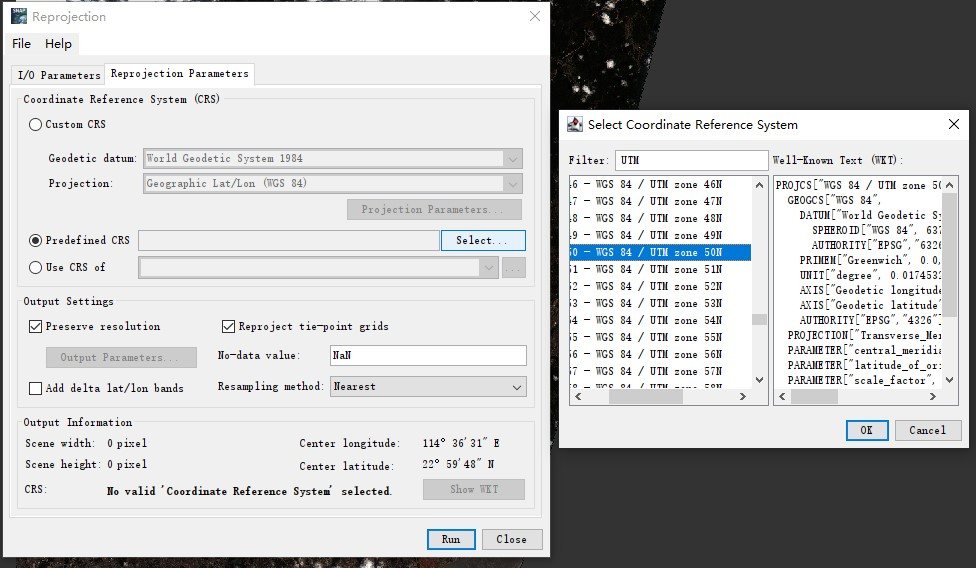
\includegraphics[height=20em]{pic/q0404.jpg}
    \caption{SNAP哨兵影像投影}
    \label{fig:0216}
\end{figure}

在ENVI中进行栅格影像重投影时, 报错如下~\ref{fig:0217}, 猜想其原因是ENVI直接从投影坐标系的库中查找上述三个参数, 可能由于命名不同, 导致无法找到对应坐标系.

\begin{figure}[!htbp]
    \centering
    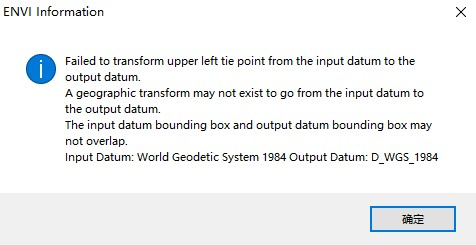
\includegraphics[height=10em]{pic/q0402.jpg}
    \caption{ENVI重投影}
    \label{fig:0217}
\end{figure}

坐标系的问题还需要再去查阅地图制图学等书籍.

% \begin{figure}[!htbp]
%     \centering
%     \subfloat[]{\label{fig:0203a}
%     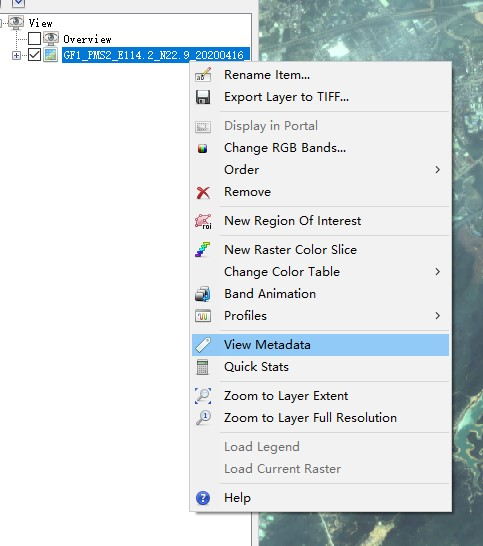
\includegraphics[height=12em]{pic/q1_02.jpg}}
%     \qquad
%     \subfloat[]{\label{fig:0203b}
%     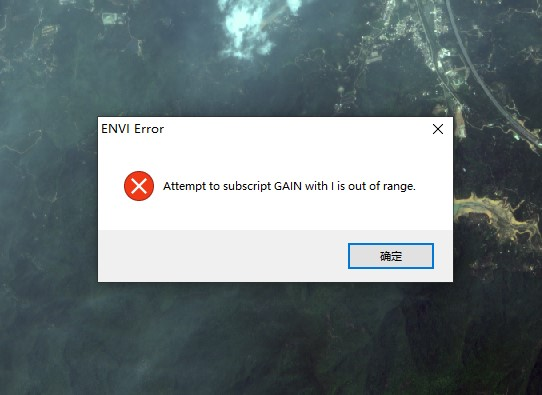
\includegraphics[height=12em]{pic/q1_04.jpg}}
%     \\[12pt]
%     \subfloat[辐射定标参数]{\label{fig:0203c}
%     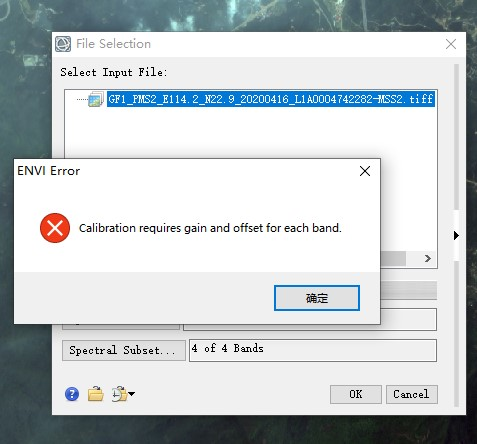
\includegraphics[height=12em]{pic/q1_03.jpg}}
%     \caption{元数据报错与辐射定标报错}
%     \label{fig:0203}
% \end{figure}

